% DO NOT COMPILE THIS FILE DIRECTLY!
% This is included by the other .tex files.

\begin{frame}[t,plain]
\titlepage
\end{frame}

\begin{frame}[t]{SirFindALot - Application Definition Statement I}

\Large
\begin{center}Sir FindALot hilft "casual" Nutzern von mobilen Endgeräten freie Parkplätze zu finden. 
Insbesondere werden auch konkret die jeweiligen freien Stellplätze auf einem ausgewählten 
Parkplatz - basierend auf (kollaborativen) Live-Daten - visuell dargestellt.
\end{center}
\end{frame}

\begin{frame}[t]{SirFindALot - Application Definition Statement II}
\Large
\begin{center}Mithilfe von Geolocation und kollaborativen Live-Daten wird eine intuitive Bedienung 
gewährleistet. Der Benutzer kann aus einer nach Geolocation und Stellplatzsituation gerankten 
Liste von vorhandenen Parkplätzen auswählen. Informationen zur aktuellen Belegung eines 
bestimmten Parkplatzes werden je nach Situation textuell und/oder visuell angezeigt. \end{center}

\end{frame}


\begin{frame}[t,fragile]{Ziele}
\begin{itemize}
\item Einfache Bedienung -- Große Buttons (während Autofahrt)
\item Wenig Klicks nötig
\item Intuitives Design und Menüführung
\end{itemize}
\end{frame}

\begin{frame}[t,fragile]{Umsetzung}
\begin{itemize}
	\item Clientseitig
		\begin{itemize}
			\item Bisher bei HTML5 (Geolocation)
			\item JavaScript Framework JQueryMobile verworfen, da nicht flüssig
			\item Eigenentwicklung JavaScript (Basis evtl JQuery oder XUI)
		\end{itemize}
	\item Serverseitig
		\textbf{Ruby on Rails} 
\end{itemize}
\end{frame}

\begin{frame}[t,fragile]{Milestones}
	Milestoneplanung:
	\begin{description}
		\item[M1: 25.11.2011] Fertiges Mobile UI Design + Javascript Framework
		\item[M2: 16.12.2011] Serverseitiges Datenbank Schema und Enwurf sowie Tests
		\item[M3: 22.12.2011] Anbindung des Mobile UI an Serverseitige Applikation
		\item[M4: 20.01.2012] Data Provider Schnittstelle + Parkplatzsimulator
	\end{description}
\end{frame}


\begin{frame}[t,fragile]{Showcases}
\begin{center}
	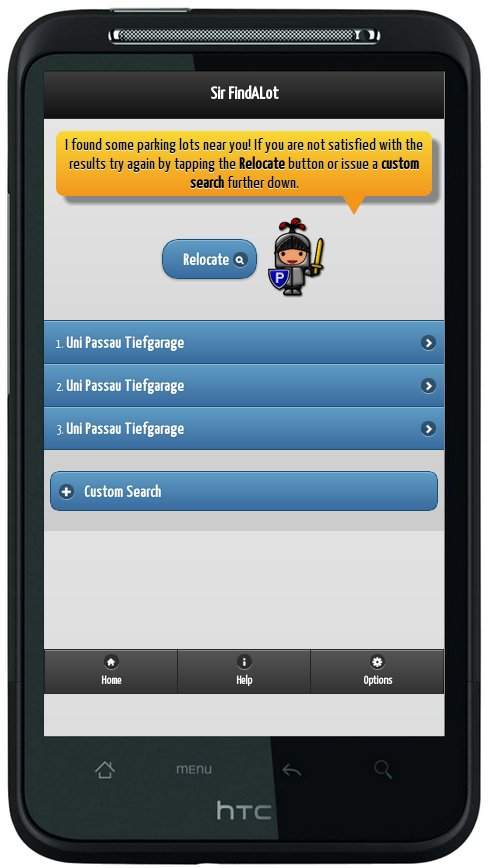
\includegraphics[width=3cm]{screen_1.jpg}
	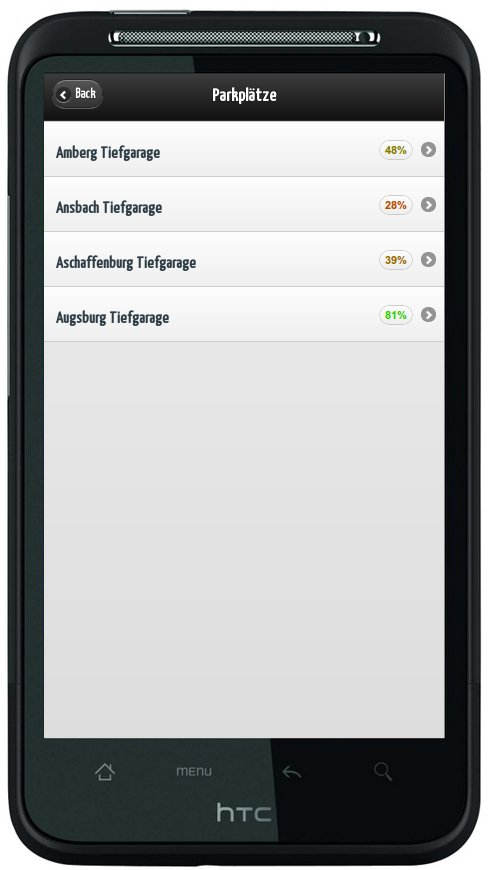
\includegraphics[width=3cm]{screen_3.jpg}
	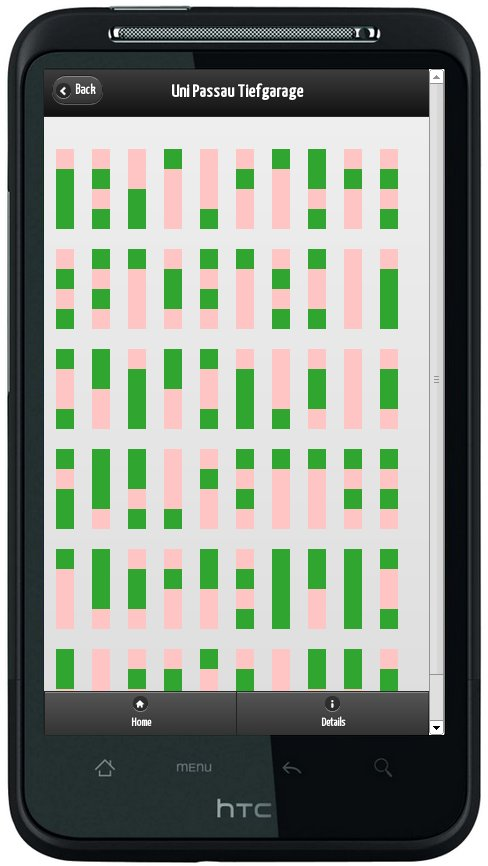
\includegraphics[width=3cm]{screen_2.jpg}
\end{center}

\end{frame}


